
%% bare_conf.tex
%% V1.3
%% 2007/01/11
%% by Michael Shell
%% See:
%% http://www.michaelshell.org/
%% for current contact information.
%%
%% This is a skeleton file demonstrating the use of IEEEtran.cls
%% (requires IEEEtran.cls version 1.7 or later) with an IEEE conference paper.
%%
%% Support sites:
%% http://www.michaelshell.org/tex/ieeetran/
%% http://www.ctan.org/tex-archive/macros/latex/contrib/IEEEtran/
%% and
%% http://www.ieee.org/

%%*************************************************************************
%% Legal Notice:
%% This code is offered as-is without any warranty either expressed or
%% implied; without even the implied warranty of MERCHANTABILITY or
%% FITNESS FOR A PARTICULAR PURPOSE! 
%% User assumes all risk.
%% In no event shall IEEE or any contributor to this code be liable for
%% any damages or losses, including, but not limited to, incidental,
%% consequential, or any other damages, resulting from the use or misuse
%% of any information contained here.
%%
%% All comments are the opinions of their respective authors and are not
%% necessarily endorsed by the IEEE.
%%
%% This work is distributed under the LaTeX Project Public License (LPPL)
%% ( http://www.latex-project.org/ ) version 1.3, and may be freely used,
%% distributed and modified. A copy of the LPPL, version 1.3, is included
%% in the base LaTeX documentation of all distributions of LaTeX released
%% 2003/12/01 or later.
%% Retain all contribution notices and credits.
%% ** Modified files should be clearly indicated as such, including  **
%% ** renaming them and changing author support contact information. **
%%
%% File list of work: IEEEtran.cls, IEEEtran_HOWTO.pdf, bare_adv.tex,
%%                    bare_conf.tex, bare_jrnl.tex, bare_jrnl_compsoc.tex
%%*************************************************************************

% *** Authors should verify (and, if needed, correct) their LaTeX system  ***
% *** with the testflow diagnostic prior to trusting their LaTeX platform ***
% *** with production work. IEEE's font choices can trigger bugs that do  ***
% *** not appear when using other class files.                            ***
% The testflow support page is at:
% http://www.michaelshell.org/tex/testflow/



% Note that the a4paper option is mainly intended so that authors in
% countries using A4 can easily print to A4 and see how their papers will
% look in print - the typesetting of the document will not typically be
% affected with changes in paper size (but the bottom and side margins will).
% Use the testflow package mentioned above to verify correct handling of
% both paper sizes by the user's LaTeX system.
%
% Also note that the "draftcls" or "draftclsnofoot", not "draft", option
% should be used if it is desired that the figures are to be displayed in
% draft mode.
%
\documentclass[conference]{IEEEtran}
%\usepackage[latin2]{inputenc}

\usepackage[utf8]{inputenc}
\usepackage[T1]{fontenc}
\usepackage{a4wide}
\usepackage{listings}
  \usepackage{courier}
 \lstset{
         basicstyle=\footnotesize\ttfamily, % Standardschrift
         %numbers=left,               % Ort der Zeilennummern
         numberstyle=\tiny,          % Stil der Zeilennummern
         %stepnumber=2,               % Abstand zwischen den Zeilennummern
         numbersep=5pt,              % Abstand der Nummern zum Text
         tabsize=2,                  % Groesse von Tabs
         extendedchars=true,         %
         breaklines=true,            % Zeilen werden Umgebrochen
         keywordstyle=\color{red},
         %       frame=b,         
 %        keywordstyle=[1]\textbf,    % Stil der Keywords
 %        keywordstyle=[2]\textbf,    %
 %        keywordstyle=[3]\textbf,    %
 %        keywordstyle=[4]\textbf,   \sqrt{\sqrt{}} %
         stringstyle=\color{white}\ttfamily, % Farbe der String
         showspaces=false,           % Leerzeichen anzeigen ?
         showtabs=false,             % Tabs anzeigen ?
         xleftmargin=17pt,
         framexleftmargin=17pt,
         framexrightmargin=5pt,
         framexbottommargin=4pt,
         %backgroundcolor=\color{lightgray},
         showstringspaces=false      % Leerzeichen in Strings anzeigen ?        
 }
 \lstloadlanguages{% Check Dokumentation for further languages ...
         %[Visual]Basic
         %Pascal
         %C
         %C++
         %XML
         %HTML
         Lisp
 }
 


  %\captionsetup[lstlisting]{singlelinecheck=false, labelfont={blue}, textfont={blue}}
 % \usepackage{caption}
%\DeclareCaptionFont{white}{\color{white}}
%\DeclareCaptionFormat{listing}{\colorbox[cmyk]{0.43, 0.35,
%0.35,0.01}{\parbox{\textwidth}{\hspace{15pt}#1#2#3}}}
%\captionsetup[lstlisting]{format=listing,labelfont=white,textfont=white,
%singlelinecheck=false, margin=0pt, font={bf,footnotesize}}

\newcommand\uv[1]{\quotedblbase #1\textquotedblleft}%
\usepackage[pdftex]{graphicx}
\graphicspath{/img/}
\DeclareGraphicsExtensions{.pdf,.jpeg,.jpg,.png}
% Add the compsoc option for Computer Society conferences.
%
% If IEEEtran.cls has not been installed into the LaTeX system files,
% manually specify the path to it like:
% \documentclass[conference]{../sty/IEEEtran}





% Some very useful LaTeX packages include:
% (uncomment the ones you want to load)


% *** MISC UTILITY PACKAGES ***
%
%\usepackage{ifpdf}
% Heiko Oberdiek's ifpdf.sty is very useful if you need conditional
% compilation based on whether the output is pdf or dvi.
% usage:
% \ifpdf
%   % pdf code
% \else
%   % dvi code
% \fi
% The latest version of ifpdf.sty can be obtained from:
% http://www.ctan.org/tex-archive/macros/latex/contrib/oberdiek/
% Also, note that IEEEtran.cls V1.7 and later provides a builtin
% \ifCLASSINFOpdf conditional that works the same way.
% When switching from latex to pdflatex and vice-versa, the compiler may
% have to be run twice to clear warning/error messages.






% *** CITATION PACKAGES ***
%
\usepackage{cite}
% cite.sty was written by Donald Arseneau
% V1.6 and later of IEEEtran pre-defines the format of the cite.sty package
% \cite{} output to follow that of IEEE. Loading the cite package will
% result in citation numbers being automatically sorted and properly
% "compressed/ranged". e.g., [1], [9], [2], [7], [5], [6] without using
% cite.sty will become [1], [2], [5]--[7], [9] using cite.sty. cite.sty's
% \cite will automatically add leading space, if needed. Use cite.sty's
% noadjust option (cite.sty V3.8 and later) if you want to turn this off.
% cite.sty is already installed on most LaTeX systems. Be sure and use
% version 4.0 (2003-05-27) and later if using hyperref.sty. cite.sty does
% not currently provide for hyperlinked citations.
% The latest version can be obtained at:
% http://www.ctan.org/tex-archive/macros/latex/contrib/cite/
% The documentation is contained in the cite.sty file itself.






% *** GRAPHICS RELATED PACKAGES ***
%
\ifCLASSINFOpdf
  % \usepackage[pdftex]{graphicx}
  % declare the path(s) where your graphic files are
  % \graphicspath{{../pdf/}{../jpeg/}}
  % and their extensions so you won't have to specify these with
  % every instance of \includegraphics
  % \DeclareGraphicsExtensions{.pdf,.jpeg,.png}
\else
  % or other class option (dvipsone, dvipdf, if not using dvips). graphicx
  % will default to the driver specified in the system graphics.cfg if no
  % driver is specified.
  % \usepackage[dvips]{graphicx}
  % declare the path(s) where your graphic files are
  % \graphicspath{{../eps/}}
  % and their extensions so you won't have to specify these with
  % every instance of \includegraphics
  % \DeclareGraphicsExtensions{.eps}
\fi
% graphicx was written by David Carlisle and Sebastian Rahtz. It is
% required if you want graphics, photos, etc. graphicx.sty is already
% installed on most LaTeX systems. The latest version and documentation can
% be obtained at: 
% http://www.ctan.org/tex-archive/macros/latex/required/graphics/
% Another good source of documentation is "Using Imported Graphics in
% LaTeX2e" by Keith Reckdahl which can be found as epslatex.ps or
% epslatex.pdf at: http://www.ctan.org/tex-archive/info/
%
% latex, and pdflatex in dvi mode, support graphics in encapsulated
% postscript (.eps) format. pdflatex in pdf mode supports graphics
% in .pdf, .jpeg, .png and .mps (metapost) formats. Users should ensure
% that all non-photo figures use a vector format (.eps, .pdf, .mps) and
% not a bitmapped formats (.jpeg, .png). IEEE frowns on bitmapped formats
% which can result in "jaggedy"/blurry rendering of lines and letters as
% well as large increases in file sizes.
%
% You can find documentation about the pdfTeX application at:
% http://www.tug.org/applications/pdftex





% *** MATH PACKAGES ***
%
%\usepackage[cmex10]{amsmath}
% A popular package from the American Mathematical Society that provides
% many useful and powerful commands for dealing with mathematics. If using
% it, be sure to load this package with the cmex10 option to ensure that
% only type 1 fonts will utilized at all point sizes. Without this option,
% it is possible that some math symbols, particularly those within
% footnotes, will be rendered in bitmap form which will result in a
% document that can not be IEEE Xplore compliant!
%
% Also, note that the amsmath package sets \interdisplaylinepenalty to 10000
% thus preventing page breaks from occurring within multiline equations. Use:
%\interdisplaylinepenalty=2500
% after loading amsmath to restore such page breaks as IEEEtran.cls normally
% does. amsmath.sty is already installed on most LaTeX systems. The latest
% version and documentation can be obtained at:
% http://www.ctan.org/tex-archive/macros/latex/required/amslatex/math/





% *** SPECIALIZED LIST PACKAGES ***
%
%\usepackage{algorithmic}
% algorithmic.sty was written by Peter Williams and Rogerio Brito.
% This package provides an algorithmic environment fo describing algorithms.
% You can use the algorithmic environment in-text or within a figure
% environment to provide for a floating algorithm. Do NOT use the algorithm
% floating environment provided by algorithm.sty (by the same authors) or
% algorithm2e.sty (by Christophe Fiorio) as IEEE does not use dedicated
% algorithm float types and packages that provide these will not provide
% correct IEEE style captions. The latest version and documentation of
% algorithmic.sty can be obtained at:
% http://www.ctan.org/tex-archive/macros/latex/contrib/algorithms/
% There is also a support site at:
% http://algorithms.berlios.de/index.html
% Also of interest may be the (relatively newer and more customizable)
% algorithmicx.sty package by Szasz Janos:
% http://www.ctan.org/tex-archive/macros/latex/contrib/algorithmicx/




% *** ALIGNMENT PACKAGES ***
%
%\usepackage{array}
% Frank Mittelbach's and David Carlisle's array.sty patches and improves
% the standard LaTeX2e array and tabular environments to provide better
% appearance and additional user controls. As the default LaTeX2e table
% generation code is lacking to the point of almost being broken with
% respect to the quality of the end results, all users are strongly
% advised to use an enhanced (at the very least that provided by array.sty)
% set of table tools. array.sty is already installed on most systems. The
% latest version and documentation can be obtained at:
% http://www.ctan.org/tex-archive/macros/latex/required/tools/


%\usepackage{mdwmath}
%\usepackage{mdwtab}
% Also highly recommended is Mark Wooding's extremely powerful MDW tools,
% especially mdwmath.sty and mdwtab.sty which are used to format equations
% and tables, respectively. The MDWtools set is already installed on most
% LaTeX systems. The lastest version and documentation is available at:
% http://www.ctan.org/tex-archive/macros/latex/contrib/mdwtools/


% IEEEtran contains the IEEEeqnarray family of commands that can be used to
% generate multiline equations as well as matrices, tables, etc., of high
% quality.


%\usepackage{eqparbox}
% Also of notable interest is Scott Pakin's eqparbox package for creating
% (automatically sized) equal width boxes - aka "natural width parboxes".
% Available at:
% http://www.ctan.org/tex-archive/macros/latex/contrib/eqparbox/





% *** SUBFIGURE PACKAGES ***
%\usepackage[tight,footnotesize]{subfigure}
% subfigure.sty was written by Steven Douglas Cochran. This package makes it
% easy to put subfigures in your figures. e.g., "Figure 1a and 1b". For IEEE
% work, it is a good idea to load it with the tight package option to reduce
% the amount of white space around the subfigures. subfigure.sty is already
% installed on most LaTeX systems. The latest version and documentation can
% be obtained at:
% http://www.ctan.org/tex-archive/obsolete/macros/latex/contrib/subfigure/
% subfigure.sty has been superceeded by subfig.sty.



%\usepackage[caption=false]{caption}
%\usepackage[font=footnotesize]{subfig}
% subfig.sty, also written by Steven Douglas Cochran, is the modern
% replacement for subfigure.sty. However, subfig.sty requires and
% automatically loads Axel Sommerfeldt's caption.sty which will override
% IEEEtran.cls handling of captions and this will result in nonIEEE style
% figure/table captions. To prevent this problem, be sure and preload
% caption.sty with its "caption=false" package option. This is will preserve
% IEEEtran.cls handing of captions. Version 1.3 (2005/06/28) and later 
% (recommended due to many improvements over 1.2) of subfig.sty supports
% the caption=false option directly:
%\usepackage[caption=false,font=footnotesize]{subfig}
%
% The latest version and documentation can be obtained at:
% http://www.ctan.org/tex-archive/macros/latex/contrib/subfig/
% The latest version and documentation of caption.sty can be obtained at:
% http://www.ctan.org/tex-archive/macros/latex/contrib/caption/




% *** FLOAT PACKAGES ***
%
%\usepackage{fixltx2e}
% fixltx2e, the successor to the earlier fix2col.sty, was written by
% Frank Mittelbach and David Carlisle. This package corrects a few problems
% in the LaTeX2e kernel, the most notable of which is that in current
% LaTeX2e releases, the ordering of single and double column floats is not
% guaranteed to be preserved. Thus, an unpatched LaTeX2e can allow a
% single column figure to be placed prior to an earlier double column
% figure. The latest version and documentation can be found at:
% http://www.ctan.org/tex-archive/macros/latex/base/



%\usepackage{stfloats}
% stfloats.sty was written by Sigitas Tolusis. This package gives LaTeX2e
% the ability to do double column floats at the bottom of the page as well
% as the top. (e.g., "\begin{figure*}[!b]" is not normally possible in
% LaTeX2e). It also provides a command:
%\fnbelowfloat
% to enable the placement of footnotes below bottom floats (the standard
% LaTeX2e kernel puts them above bottom floats). This is an invasive package
% which rewrites many portions of the LaTeX2e float routines. It may not work
% with other packages that modify the LaTeX2e float routines. The latest
% version and documentation can be obtained at:
% http://www.ctan.org/tex-archive/macros/latex/contrib/sttools/
% Documentation is contained in the stfloats.sty comments as well as in the
% presfull.pdf file. Do not use the stfloats baselinefloat ability as IEEE
% does not allow \baselineskip to stretch. Authors submitting work to the
% IEEE should note that IEEE rarely uses double column equations and
% that authors should try to avoid such use. Do not be tempted to use the
% cuted.sty or midfloat.sty packages (also by Sigitas Tolusis) as IEEE does
% not format its papers in such ways.





% *** PDF, URL AND HYPERLINK PACKAGES ***
%
%\usepackage{url}
% url.sty was written by Donald Arseneau. It provides better support for
% handling and breaking URLs. url.sty is already installed on most LaTeX
% systems. The latest version can be obtained at:
% http://www.ctan.org/tex-archive/macros/latex/contrib/misc/
% Read the url.sty source comments for usage information. Basically,
% \url{my_url_here}.





% *** Do not adjust lengths that control margins, column widths, etc. ***
% *** Do not use packages that alter fonts (such as pslatex).         ***
% There should be no need to do such things with IEEEtran.cls V1.6 and later.
% (Unless specifically asked to do so by the journal or conference you plan
% to submit to, of course. )


% correct bad hyphenation here
\hyphenation{op-tical net-works semi-conduc-tor}


\begin{document}
%
% paper title
% can use linebreaks \\ within to get better formatting as desired
\title{Unifying execution of imperative and declarative code}


% author names and affiliations
% use a multiple column layout for up to three different
% affiliations
\author{\IEEEauthorblockN{Martin Kožený}
\IEEEauthorblockA{Faculty of Informatics\\
Czech Technical University in Prague\\
Czech Repuplic\\
Email: martin.kozeny@gmail.com}
}

% conference papers do not typically use \thanks and this command
% is locked out in conference mode. If really needed, such as for
% the acknowledgment of grants, issue a \IEEEoverridecommandlockouts
% after \documentclass

% for over three affiliations, or if they all won't fit within the width
% of the page, use this alternative format:
% 
%\author{\IEEEauthorblockN{Michael Shell\IEEEauthorrefmark{1},
%Homer Simpson\IEEEauthorrefmark{2},
%James Kirk\IEEEauthorrefmark{3}, 
%Montgomery Scott\IEEEauthorrefmark{3} and
%Eldon Tyrell\IEEEauthorrefmark{4}}
%\IEEEauthorblockA{\IEEEauthorrefmark{1}School of Electrical and Computer Engineering\\
%Georgia Institute of Technology,
%Atlanta, Georgia 30332--0250\\ Email: see http://www.michaelshell.org/contact.html}
%\IEEEauthorblockA{\IEEEauthorrefmark{2}Twentieth Century Fox, Springfield, USA\\
%Email: homer@thesimpsons.com}
%\IEEEauthorblockA{\IEEEauthorrefmark{3}Starfleet Academy, San Francisco, California 96678-2391\\
%Telephone: (800) 555--1212, Fax: (888) 555--1212}
%\IEEEauthorblockA{\IEEEauthorrefmark{4}Tyrell Inc., 123 Replicant Street, Los Angeles, California 90210--4321}}




% use for special paper notices
%\IEEEspecialpapernotice{(Invited Paper)}




% make the title area
%\maketitle
\maketitle

\begin{abstract}
%\boldmath
Using unified environment for both imperative and declarative code is quite
interesting point of view on programming these days. Why is it interesting?
Obviously by ability of mixing imperative and declarative code can programmer
easily express constraints of problem using declarative code in terms of
existing data structures in imperative programming. This give us very strong
tool to solve easily problems, which are especially in imperative programming
difficult to solve.
\end{abstract}
% IEEEtran.cls defaults to using nonbold math in the Abstract.
% This preserves the distinction between vectors and scalars. However,
% if the conference you are submitting to favors bold math in the abstract,
% then you can use LaTeX's standard command \boldmath at the very start
% of the abstract to achieve this. Many IEEE journals/conferences frown on
% math in the abstract anyway.

% no keywords




% For peer review papers, you can put extra information on the cover
% page as needed:
% \ifCLASSOPTIONpeerreview
% \begin{center} \bfseries EDICS Category: 3-BBND \end{center}
% \fi
%
% For peerreview papers, this IEEEtran command inserts a page break and
% creates the second title. It will be ignored for other modes.
\IEEEpeerreviewmaketitle



\section{Introduction}
Motivation for writing this paper is to present unconventional way of
programming, show how it works and its advantages and disadvantages and
sketch its possible development in the future.

First question when solving problem of unified execution environment is how to
mix declarative and programming paradigms together. What are the possibilities
of interleaving or cooperating between these two paradigms. Regarding this
issue, there are two different attitudes.

First one is Java framework Squander developed at Massachusetts Institute of
Technology by Mr. Aleksandar Milicevic. This framework implements declarative
paradigm in prgramming language Java using annotations. Via those annotations
can programmer declare preconditions of heap state, part of the heap, which is
allowed to modify and how should objects on heap look like after execution.


Another approach provides Jess rule engine. This engine was entirely written by
Ernest Friedman-Hill at Sandia National Laboratories in Livermore, CA. Jess uses
enhanced version of the Rete algorithm to process rules. Rete is a very
efficient mechanism for solving the difficult many-to-many matching problem.
Jess engine consist of working memory representing set of facts and rules for
manipulating with those facts. Engine can directly access Java objects,
invoke methods or implement interfaces.

\section{Framework Squander}
Squander is a framework that provides a unified environment for writing
declarative constraints and imperative statements in the context of a single
program. This is particularly useful for implementing programs that involve
computations that are relatively easy to specify but hard to solve
algorithmically\cite{milicevic:executableSpecificationsForJavaPrograms}.

Let us define execution of Squander on framework's architecture presented at
Figure \ref{fig:architecture}.

\begin{figure}[ht]
\begin{center}
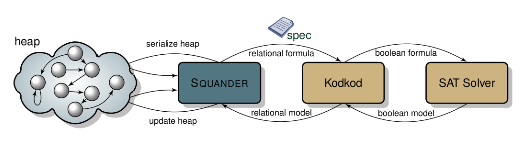
\includegraphics[width=7cm]{img/architecture-diagram}
\caption{Architecture diagram}
\label{fig:architecture}
\end{center}
\end{figure}

Excution of Squander is defined by following steps\cite{web:squander}:
\begin{enumerate}
  \item serialize heap into relations
  \item translate specs and heap relations into Kodkod
  \item translate relational into boolean logic
  \item (if a solution is found) restore relations from boolean assignments
  (if a solution is found) restore field values from relations
  \item (if a solution is found) restore the heap to reflect the solution
   
\end{enumerate}



Main terms defining this framework are Kodkod and JSFL. 

Kodkod is a solver for relational logic. Kodkod requires bounded universe, a  et
of untyped relations, bounds for every relation and relation formula. Then
translates given problem into boolean satisfiability problem (SAT) and applies
of-the-shelf SAT solver to search for satisfying solution, which is reflected
back if found.

JSFL is formal lightweight specification for Java supporting relational and set
algebra, as well as common Java operators. Using expressive power of relation
algebra, JFSL makes it easy to succinctly and formally specify complex
properties about Java programs such as method pre and postcondition, class
invariants and so called frame conditions, which means portion of the heap, that
is methods allow to modify. It also supports specification fields
which can be useful for specifying abstract data types.

 
\section{Jess}
This section is written using Jess manual\cite{jess:manual}.


Jess is a rule engine and scripting environment using form
of declarative rules and is a highly specialized form of Lisp. The payoff of
this engine is that it is very expressive, and can implement complex logical
relationships with very little code.

In Jess everything is a function call. Each Jess rule engine holds a collection
of knowledge nuggets called facts. This collection is known as the working
memory. Working memory is important because rules can only react to additions,
deletions, and changes to working memory. You cannot write a Jess rule that will
react to anything else.



In Jess, there are three kinds of facts: unordered facts, shadow facts and
ordered facts. Unordered facts provide slots, where data appeared similarly like
fields in Java objects. Shadow facts are connected to Java objects, so by using
shadow facts is possible to put any Java object into Jess's working memory. In
that way, template for the fact is created by looking at a Java class.
When some property of the Java object respectively Jess fact is changed, it is
necessary to explicitly notify Jess fact respectively Java object about this
change. Ordered facts are simply Jess lists, where the first field (the head of
the list) acts as a sort of category for the fact. 




Rules are used to search the facts to find relationships
between them, and also can take actions based on the contents of one or more
facts. A Jess rule is something like an \textit{if then statement} in a
procedural language, but it is not used in a procedural way. While if... then statements are executed at a specific time and in a
specific order, according to how the programmer writes them, Jess rules are executed
whenever their if parts (their left-hand-sides or LHSs) are satisfied, given only that the rule
engine is running. This makes Jess rules less deterministic than a typical procedural program.


The obvious implementation for the rule engine is very inefficient. This
implementation would be to keep a list of the rules and continuously cycle
through the list, checking each one's left-hand-side (LHS) against the working
memory and executing the right-hand-side (RHS) of any rules that apply. This is
inefficient because most of the tests made on each cycle will have the same
results as on the previous iteration. However, since the working memory is
stable, most of the tests will be repeated. You might call this the rules
finding facts approach and its computational complexity is of the order of
$O(R.F^P)$, where $R$ is the number of rules, $P$ is the average number of
patterns per rule LHS, and $F$ is the number of facts on the working memory.



Architecture can be many orders of magnitude faster than an equivalent set
of traditional if... then statements. This is caused by using RETE Match
algorithm for pattern matching, where the inefficiency described above is
alleviated by remembering past test results across iterations of the rule
loop.Only new facts are tested against any rule LHSs. Additionally, as will be
described below, new facts are tested against only the rule LHSs to which they
are most likely to be relevant. As a result, the computational complexity per
iteration drops to something more like $O(R.F.P)$, or linear in the size of
working memory.



Jess rules has two parts. The first part consists of the LHS pattern. The second
part consists of the RHS action, which is executed, when LHS part of the rule is fullfilled. LHS of a
rule consists of patterns which are used to match facts in the working memory,
while the RHS contains function calls. The LHS of a rule (the "if" part)
consists of patterns that match facts. The actions of a rule (the "then" clause)
are made up of function calls.





%Some facts are pure facts defined and
%created entirely by Jess. Other facts are shadow facts connected to Java
%objects you provide. Shadow facts act as "bridges" that let Jess reason about
%things that happen outside of working memory. Every fact has a template. The
%template has a name and a set of slots, and each fact gets these things from
%its template. This is the same structure that JavaBeans -- plain old Java
%objects, or POJOs -- have, and it's also similar to how relational databases
%are set up. The template is like the class of a Java object, or like a
%relational database table. The slots are like the properties of the JavaBean,
%or the columns of a table. A fact is therefore like a single JavaBean, or like
%a row in a database table. You can think of it either way. In Jess, there are
%three kinds of facts: unordered facts, shadow facts and ordered facts.

%Unordered facts
%In object-oriented languages like Java, objects have named fields in which data
%appears. Unordered facts offer this capability (although the fields are
%traditionally called slots.)

%Ordered facts
%Most of the time, you will use unordered facts (or their cousins, shadow
%facts.) They are nicely structured, and they're the most efficient kind of fact
%in Jess. In some cases, though, slot names are redundant, and force you to do
%more typing than you'd like. For example, if a fact represents a single number,
%it seems silly to use an unordered fact like this:

%Rules
%Now that we've learned how to populate Jess's working memory, we can answer the
%obvious question: what is it good for? The answer is that defquerys can search
%it to find relationships between facts, and defrules can take actions based on
%the contents of one or more facts. A Jess rule is something like an if... then
%statement in a procedural language, but it is not used in a procedural way.
%While if... then statements are executed at a specific time and in a specific
%order, according to how the programmer writes them, Jess rules are executed
%whenever their if parts (their left-hand-sides or LHSs) are satisfied, given
%only that the rule engine is running. This makes Jess rules less deterministic
%than a typical procedural program. See the chapter on the Rete algorithm for an
%explanation of why this architecture can be many orders of magnitude faster
%than an equivalent set of traditional if... then statements. In this chapter
%we're going to make a lot of use of a "person" template that looks like this:



%This rule has two parts, separated by the "=>" symbol (which you can read as
%"then".) The first part consists of the LHS pattern (person {age < 3}). The
%second part consists of the RHS action, the call to println. If you're new to
%Jess, it can be hard to tell the difference due to the LISP-like syntax, but
%the LHS of a rule consists of patterns which are used to match facts in the
%working memory, while the RHS contains function calls. The LHS of a rule (the
%"if" part) consists of patterns that match facts, NOT function calls. The
%actions of a rule (the "then" clause) are made up of function calls. The
%following rule does NOT


\section{Conclusion}
This paper describes different approaches of implementation of unified
environment for declarative and imperative code. Framework Squander provides
this environment using Java built in annotations whereas Jess uses special
scripting environment. Main difference is that Jess rules engine was primary
developed for building complicated expert systems\cite{hill:jessInAction} like diagnostic systems
whereas Squander was invented for solving hard constraint problems or generate
data structure instances satisfying complex constraints. Moreover Sqaunder was
developed in recent years and nowadays is used for further academic research of
this topic but Jess was written almost twenty years ago and many systems was
developed using this engine.


\begin{thebibliography}{1}

\bibitem{milicevic:executableSpecificationsForJavaPrograms}
Aleksandar Milicevic; MASSACHUSETTS INSTITUTE OF TECHNOLOGY, Department of
Electrical Engineering and Computer Science; \textit{Executable Specifications
for Java Programs}, September 2010.



\bibitem{web:squander}Squander
official website;\\\verb|http://people.csail.mit.edu/aleks/squander/|


\bibitem{hill:jessInAction}
Ernst Friedman-Hill; \textit{Jess in Action}, September 2003.



\bibitem{jess:manual}Jess official
website;\\\verb|http://www.jessrules.com/jess/docs/71/|




\end{thebibliography}




% that's all folks
\end{document}

